\documentclass{article}
\usepackage[a4paper, margin=1in]{geometry}
\usepackage[T1]{fontenc}
\usepackage[utf8]{inputenc}
\usepackage{amsmath, amssymb, graphicx, hyperref}
\usepackage{bookmark}
\graphicspath{{../figures/}}
\usepackage[framed,numbered]{matlab-prettifier}
\usepackage{xcolor}
\usepackage{listings}

\geometry{a4paper, margin=1in}

% MATLAB code style
\lstset{
  style      = Matlab-editor,
  basicstyle = \mlttfamily,
  breaklines = true
}

\title{\textbf{{Practical - 10}}}
\author{}
\date{October 29, 2026}

\pagenumbering{gobble}

\begin{document}
\maketitle

\noindent
\textbf{\large{Aim:}} To analyze the basic Lotka-Volterra predator-prey model and plot the populations of prey and predators over time.

\vspace{1em}
\noindent
\textbf{\large{Theory:}}

\vspace{0.5em}
\noindent
\textbf{Basic Concept}

\noindent
The predator–prey model describes the interaction between two populations. The prey (for example: rabbit) is hunted by the predator (for example: fox), while the predator depends on the prey for food.
\begin{itemize}
    \item Without predators, prey grow naturally.
    \item Without prey, predators decline because food is unavailable.
    \item More prey can support predator growth.
    \item More predators increase the rate at which prey is consumed.
\end{itemize}

\vspace{0.5em}
\noindent
\textbf{Mathematical model}

\noindent
Let $x(t)$ denote the prey population and $y(t)$ denote the predator population at time $t$. The basic Lotka–Volterra model is:
\[\frac{dx}{dt} = ax - bxy\]
\[\frac{dy}{dt} = cxy - dy\]
where $a, b, c$ and $d$ are positive constants.

\begin{table}[h]
    \centering
    \begin{tabular}{|c|c|}
    \hline
    \textbf{Parameter} & \textbf{Meaning} \\
    \hline
    \textbf{$a$} & Natural growth rate of prey \\
    \hline
    \textbf{$b$} & Rate at which predators consume prey \\
    \hline
    \textbf{$c$} & Rate at which feeding supports predator growth \\
    \hline
    \textbf{$d$} & Natural death rate of predators \\
    \hline
    \end{tabular}
\end{table}

\vspace{0.5em}
\noindent
\textbf{Understanding the Equations}

\noindent
Prey: $\frac{dx}{dt} = ax - bxy$. The term $ax$ represents natural prey growth, and $-bxy$ represents prey loss due to predator attacks.

\noindent
Predator: $\frac{dy}{dt} = cxy - dy$. The term $cxy$ represents predator growth supported by feeding, and $-dy$ represents natural predator deaths.

\noindent
The product $xy$ represents interactions between the two populations.

\newpage
\noindent
\textbf{\large{MATLAB Code:}}
\begin{lstlisting}
clc; clear all; close all;

a = 1.0;
b = 0.1;
c=0.075;
d=1.5;

x0 = 40; % Initial prey population
y0 = 9;  % Initial predator population

tspan = [0,30];
initial = [x0,y0];

f = @(t,z)[a*z(1)- b*z(1)*z(2);
    c*z(1)*z(2) - d*z(2)];

[t,Z] = ode45(f, tspan, initial);

x = Z(:,1);
y = Z(:,2);

plot(t, x, 'LineWidth',1.5)
hold on
plot(t, y, 'LineWidth',1.5)
grid on
xlabel('Time')
ylabel('Population')
title('Basic Lotka-Volterra Predator-Prey Model')
legend('Prey Population', 'Predator Population', 'Location','best')
hold off
\end{lstlisting}

\vspace{1em}
\noindent
\textbf{\large{Output:}}
\begin{figure}[htbp]
    \centering
    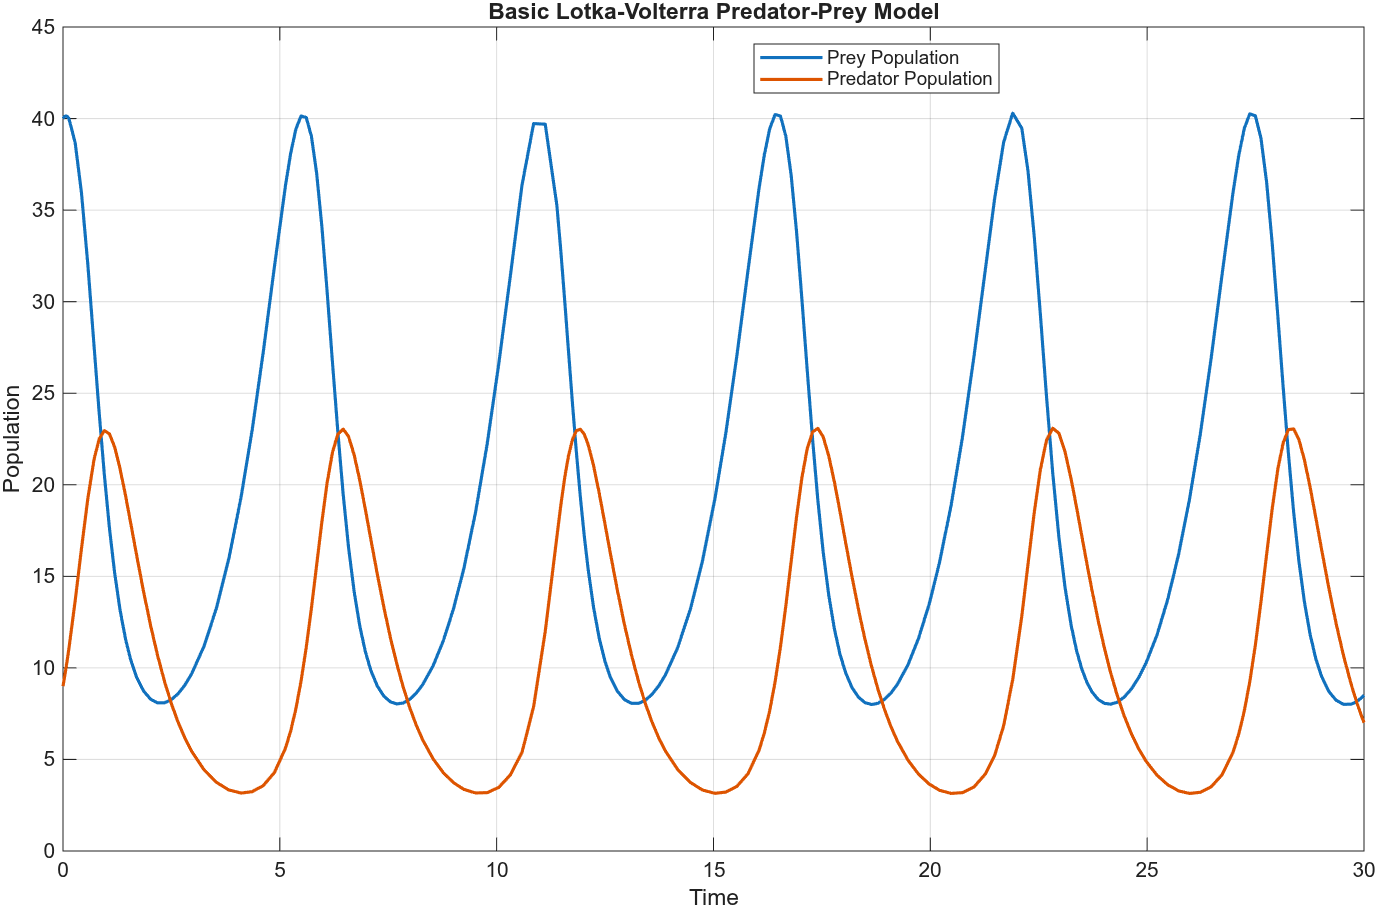
\includegraphics[width=0.7\textwidth]{Figure10.png}
\end{figure}

\newpage
\noindent
\textbf{Explanation of the MATLAB Code}
\begin{enumerate}
\item \textbf{x0 and y0 :} Specify the initial prey and predator populations.
\item \textbf{tspan = [0 30] :} Sets the time interval for solving the model.
\item \textbf{initial = [x0; y0] :} Stores both initial populations in a column vector.
\item \textbf{f = @(t,z) [...] :} Defines the two differential equations. z(1) is prey and z(2) is predator.
\item \textbf{ode45(f,tspan,initial) :} Numerically solves the coupled differential equations.
\item \textbf{Z(:,1) and Z(:,2) :} Extract the prey and predator values from the solution matrix.
\end{enumerate}

\vspace{1em}
\noindent
\textbf{Why Is ode45 used Instead of dsolve?}

\noindent
The basic Lotka-Volterra model is a nonlinear coupled system. Although dsolve is useful when a symbolic solution is available, it generally does not provide a convenient explicit time-dependent formula for this system. ode45 computes a numerical approximation at many time points so the populations can be plotted.

\vspace{1em}
\noindent
\textbf{Interpretation of the Graph}

\noindent
The populations often rise and fall in cycles in the basic model. When prey become plentiful, predator numbers may increase after them. As predator numbers rise, prey numbers may decrease. With fewer prey, predator numbers may then decline, allowing prey to recover. The precise curve depends on the parameters and initial populations.

\end{document}
